\section{Global Model Agnostic}

\subsection{PDP - Partial Dependency Plot}
\textit{On average, over all samples in the dataset, how does the prediction change,
	when we hold all but one or two features constant and replace the remaining features with values from a grid.}
\begin{itemize}
	\item Shows the marginal effect of one or two features on model predictions
	\item Detect the type of relationship (linear, monotonic or complex)
	\item Is the average of all ICE-Curves for a feature.
	\item Goal: Show how features affect the prediction on average.
	\item How the prediction changes with features in S on average.
	\item Ignores feature interactions. $\to$ low importance to features that matter via interactions
	\item Visualize global feature effects on model predictions.
	\item If features uncorrleated, interpretation is clear and accurate.
	\item Practically limited to at most two features.
	\item Gives causal interpretation for the model (not necessarily the real world)
	\item Dont show distribution of data points. Leads to overinterpreation where there is little data
	\item Alternative use ALE especailly when we have correlated features.
	\item Complement them with ALE and ICE cureves for better insights.
\end{itemize}

\begin{align}
	\hat{f}_S(\mathbf{x}_S) & = \mathbb{E}_{\mathbf{X}_C}\left[\hat{f}(\mathbf{x}_S, X_C)\right]     & = \int \hat{f}(\mathbf{x}_S, X_C) d\mathbb{P}(\mathbf{X}_C)                      \\
	\hat{f}_S(\mathbf{x}_S) & = \frac{1}{n} \sum_{i=1}^n \hat{f}(\mathbf{x}_S, \mathbf{x}^{(i)}_{C}) &                                                             & \text{Monte Carlo}
\end{align}
\begin{itemize}
	\item $x_s$ features for which the pdp should be plotted
	\item $X_C$ Other features. These are replaced by the other values in the dataset.
	\item Marginalize model output over the distribution of the features in set $C$
\end{itemize}

\begin{figure}[H]
	\begin{center}
		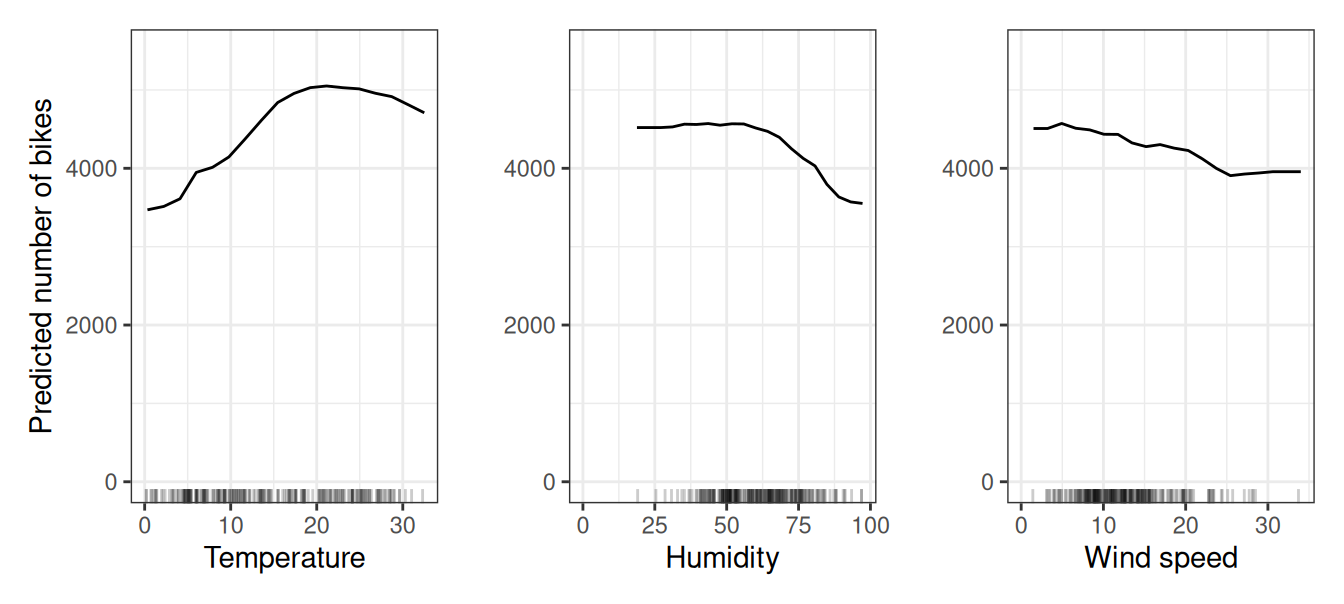
\includegraphics[width=0.8\linewidth]{images/fig-pdp-bike-1.png}
	\end{center}
	\caption{PDP example}\label{fig:pdpexample}
\end{figure}

\begin{figure}[H]
	\begin{center}
		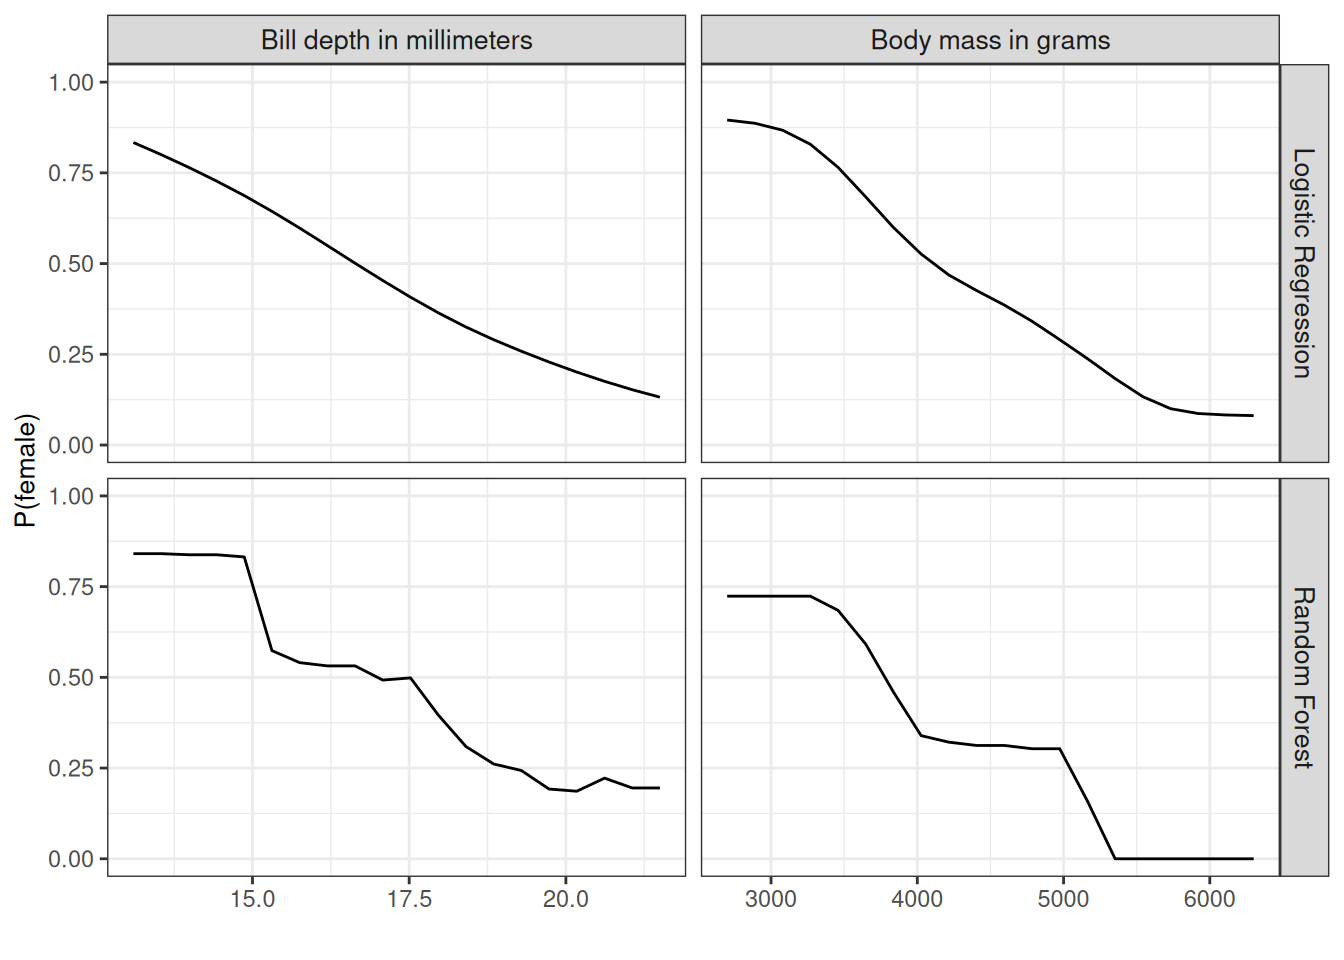
\includegraphics[width=0.8\linewidth]{images/fig-pdp-penguin-1.png}
	\end{center}
	\caption{PDP example 2}\label{fig:pdp-interactionstypes}
\end{figure}
\paragraph{Notes}
\begin{itemize}
	\item Assumes no strong correlationbetween features in S and C
	\item  If violated, unrealistic data points may be used.
	\item Works the same way for categorical. Replace all values with one class and get the average prediction.
\end{itemize}

\subsubsection{PDP Feature Importance}
\begin{itemize}
	\item Flat PDP $\to$ feature is unimportant
	\item Highly varying PDP $\to$ feature is important.
	\item If a feature is constant, it has no predictive power.
\end{itemize}
For numerical features: Importance is the standard deviation of PDP values.
\begin{equation}
	I(\mathbf{x}_S) =  \sqrt{\frac{1}{K-1}\sum_{k=1}^K\left(\hat{f}_S(\mathbf{x}^{(k)}_S) - \frac{1}{K}\sum_{k=1}^K \hat{f}_S(\mathbf{x}^{(k)}_S)\right)^2}
	\label{eq:pdpimportance}
\end{equation}
Normal distribution, 95\% of values are within $\pm 2\sigma$
